\subsection{题目描述}
\noindent
Write a MC code for a 3D Face-Centered Cubic lattice using the Heisenberg spin
model (adopt periodic boundary condition). Estimate the ferromagnetic Curie temperature.
\[
    H = -J \sum_{\langle i,j \rangle} \vec{S}_i \cdot \vec{S}_j, \quad J = 1, \quad |\vec{S}_i| = 1
\]


\subsection{程序描述}
\textit{代码尚有不少改进空间，奈何期末有心杀贼，无力回天}

程序内置以下模块：
\begin{itemize}
    \item \texttt{PhysicalQuantities.py}：管理所有的物理量与转换关系，其中比热与磁化强度均按照涨落公式计算,Binder比用于辨别相变点与性质
          \[
              C = \frac{\langle E^2 \rangle - \langle E \rangle^2}{k_B T^2}, \quad \chi = \frac{\langle M^2 \rangle - \langle M \rangle^2}{k_B T}, \quad U  = 1- \frac{\langle M^4 \rangle }{3(\langle M^2 \rangle)^2 }
          \]
          内有\texttt{to\_dict}等配套方法
    \item \texttt{HeisenbergFCC.py}：实现了一个3D面心立方晶格的海森堡模型，其中包含了初始化、构建近邻列表、测量物理量与利用FFT测量自旋关联函数以及结构因子等方法
    \item \texttt{updater.py}：内置UpdaterBase基类，下辖SingleSpinUpdate、SwendsenWangUpdate与WolffUpdate三个子类，分别实现了单自旋更新、Swendsen-Wang翻转与Wolff翻转三种更新方法，其中Swendsen-Wang与Wolff的团簇激活概率均为2D Ising模型的直接推广\footnote{Nonomura, Y. and Tomita, Y., 2015. Nonequilibrium behaviors of 3D Heisenberg model in the Swendsen-Wang algorithm. arXiv preprint \href{https://arxiv.org/abs/1508.05218}{arXiv:1508.05218.}}
          \[
              p=1-\exp[-2\beta (\overrightarrow{r}\cdot\overrightarrow{S}_i)(\overrightarrow{r}\cdot\overrightarrow{S}_j)]
          \]
          其中$\overrightarrow{r}$为每步随机选择的单位投影方向，Swendsen-Wang每次以概率$\frac{1}{2}$翻转所有团簇，Wolff随机生长并翻转
    \item \texttt{FSAnalysis.py}：有限尺寸分析模块，内含数据坍缩处理与临界温度定位，但在主程序中尚未集合运用，咕咕咕
    \item \texttt{Simulation.py}：模拟控制类，内置单温度\footnote{本程序所有温度采用$J/k_b$单位}模拟、温度区间模拟退火，均支持并行计算
    \item \texttt{Visualization.py}：可视化模块，内含自旋构型、物理量、关联函数与结构因子的可视化方法，支持动画输出
    \item \texttt{Interactive.py}：交互模块，借助PyQt5实现了一个简单的GUI，集成模拟控制与可视化功能，在终端借助\texttt{tqdm}实时输出进度条
\end{itemize}
以上模块化代码均存放在\texttt{src/modules}中，可能需要预先加载到Python环境中，为便于助教老师调试，在\texttt{src}中还放置了一个\texttt{heisenberg.py}，里面包含所有模块的代码，不便于阅读，但可在该目录直接运行\ccmd{python -u heisenberg.py}以启动交互模拟，需要安装辅助运算的库\texttt{numpy}与\texttt{scipy}，用于绘图的\texttt{matplotlib}与用于交互的\texttt{pyqt5}，以及进度条\texttt{tqdm}.
\subsection{伪代码}
Powered by \href{https://chatgpt.com/g/g-xJJAA2awf-latex-pseudocode-generator}{\LaTeX \ pseudocode generator}

\begin{algorithm}[H]
    \SetKwFunction{RandomRotation}{RandomRotation}
    \SetKwFunction{Update}{Update}
    \SetKwFunction{Sweep}{Sweep}
    \SetKwFunction{AdjustStepSize}{AdjustStepSize}
    \SetKwFunction{GetSpin}{GetSpin}
    \SetKwFunction{CalculateEnergy}{CalculateEnergy}
    \SetKwData{Model}{model}
    \SetKwData{DeltaTheta}{\(\Delta\theta_{\max}\)}
    \SetKwData{Beta}{\(\beta\)}
    \SetKwData{Proposed}{n\_proposed}
    \SetKwData{Accepted}{n\_accepted}

    \KwIn{\Model, \DeltaTheta, \Beta}
    \KwOut{Updated \Model, acceptance rate}

    \BlankLine
    \DeltaTheta $\leftarrow \min(\DeltaTheta, \pi)$\;
    \Proposed, \Accepted $\leftarrow 0, 0$\; % Initialization

    \BlankLine
    \SetKwProg{Fn}{Function}{:}{}
    \Fn{\RandomRotation{\(s\)}}{
        Sample \(\Delta \theta \sim [0, \DeltaTheta]\), unit vector \( \text{axis} \)\;
        Compute new spin via Rodrigues' formula\;
        \Return{normalized spin}
    }

    \BlankLine
    \Fn{\Update{}}{
        \(i \sim \text{Uniform}(0, \Model.N)\), \(s_{\text{old}} \leftarrow \Model.\GetSpin(i)\)\;
        \(E_{\text{old}} \leftarrow \Model.\CalculateEnergy(i)\)\;
        \(s_{\text{new}} \leftarrow \RandomRotation(s_{\text{old}})\)\;
        \(\Model.\text{spins}[i] \leftarrow s_{\text{new}}\), \(E_{\text{new}} \leftarrow \Model.\CalculateEnergy(i)\)\;
        \(\Delta E \leftarrow E_{\text{new}} - E_{\text{old}}\)\;

        \Proposed $\mathrel{+}= 1$\;
        \lIf{\(\Delta E \leq 0 \textbf{ or } e^{-\Beta \Delta E} > \text{rand}(0,1)\)}{
            \Accepted $\mathrel{+}= 1$, \Model.energy $\mathrel{+}= \Delta E$
        }
        \lElse{\(\Model.\text{spins}[i] \leftarrow s_{\text{old}}\)}
    }

    \BlankLine
    \Fn{\Sweep{}}{
        \For{\(1\) to \Model.N}{
            \Update{}\;
        }
    }

    \BlankLine
    \Fn{\AdjustStepSize{\(r_{\text{target}}, \epsilon\)}}{
        \If{\Proposed = 0}{\Return\;}
        Compute \(r = \frac{\Accepted}{\Proposed}\)\;
        \If{\(|r - r_{\text{target}}| > \epsilon\)}{
            \DeltaTheta $\mathrel{*}= r / r_{\text{target}}$, clamp to \([10^{-5}, \pi]\)\;
        }
        Reset \Proposed and \Accepted\;
    }

    \caption{Single Spin Metropolis Update}
\end{algorithm}


\begin{algorithm}[H]
    \SetKwFunction{Find}{Find}
    \SetKwFunction{Union}{Union}
    \SetKwFunction{GenerateProjectionDirection}{GenerateProjectionDirection}
    \SetKwFunction{CalculateEnergy}{CalculateEnergy}
    \SetKwFunction{ClusterFormation}{ClusterFormation}
    \SetKwFunction{ClusterUpdate}{ClusterUpdate}
    \SetKwData{Model}{model}
    \SetKwData{Labels}{labels}
    \SetKwData{ProjectionDir}{projection\_dir}
    \SetKwData{BetaJ}{$\beta J$}
    \SetKwData{Neighbors}{neighbors}

    \KwIn{\Model, \(\beta\), \(J\)}
    \KwOut{Updated \Model with new spin configuration and energy}

    \BlankLine
    \Labels $\leftarrow$ Initialize for all spins\;
    \ProjectionDir $\leftarrow$ \GenerateProjectionDirection{} \tcp*[r]{Generate random projection direction}

    \BlankLine
    \SetKwProg{Fn}{Function}{:}{}
    \Fn{\GenerateProjectionDirection{}}{
        Sample \(\mathbf{r}\) from \(\mathbb{R}^3\), \Return{\(\mathbf{r} / \|\mathbf{r}\|\)}\;
    }

    % \BlankLine
    % \Fn{\Find{\(x\)}}{
    %     \While{\(\Labels[x] \neq x\)}{\Labels[x] $\leftarrow$ \Labels[\Labels[x]], \(x \leftarrow \Labels[x]\)}\;
    %     \Return{\(x\)}
    % }

    % \BlankLine
    % \Fn{\Union{\(x, y\)}}{
    %     \(x_r, y_r \leftarrow \Find(x), \Find(y)\)\;
    %     \If{\(x_r \neq y_r\)}{\(\Labels[y_r] \leftarrow x_r\)}\;
    % }

    \BlankLine
    \SetKwProg{Subroutine}{Subroutine}{:}{}
    \Subroutine{ClusterFormation}{
        \ForEach{neighbor pair \((i, j)\) in \Neighbors}{
            \(S_i, S_j \leftarrow \Model.\text{spins}[i] \cdot \ProjectionDir, \Model.\text{spins}[j] \cdot \ProjectionDir\)\;
            \If{\(S_i S_j > 0\) and random() $< 1 - e^{-2 \cdot \BetaJ \cdot S_i S_j}$}{
                \Union{\(i, j\)}\;
            }
        }
    }

    \BlankLine
    \Subroutine{ClusterUpdate}{
        \ForEach{cluster in \Labels}{
            \If{random() $< 0.5$}{Flip all spins in the cluster along \ProjectionDir{}\;}
        }
    }

    \BlankLine
    \Fn{SwendsenWangUpdate{}}{
        Reset \Labels{} ;\ClusterFormation{} \tcp*[r]{Form clusters}
        Extract clusters from \Labels{}
        \ClusterUpdate{} \tcp*[r]{Flip clusters}
        \Model.energy $\leftarrow$ \CalculateEnergy{} \tcp*[r]{Update energy}
    }

    \caption{Swendsen-Wang Cluster Update Algorithm (Simplified)}
\end{algorithm}

\begin{algorithm}[H]
    \SetKwFunction{GenerateProjectionDirection}{GenerateProjectionDirection}
    \SetKwFunction{CalculateEnergy}{CalculateEnergy}
    \SetKwData{Model}{model}
    \SetKwData{Cluster}{cluster}
    \SetKwData{ProjectionDir}{projection\_dir}
    \SetKwData{Stack}{stack}
    \SetKwData{Neighbors}{neighbors}

    \KwIn{\Model, \(\beta\), \(J\)}
    \KwOut{Updated \Model with new spin configuration and energy}

    \BlankLine
    \SetKwProg{Fn}{Function}{:}{}
    \Fn{\GenerateProjectionDirection{}}{
        Sample random vector \(\mathbf{r}\) from \(\mathbb{R}^3\)\;
        \Return{\(\mathbf{r} / \|\mathbf{r}\|\)}\;
    }

    \BlankLine
    \Fn{WolffUpdate{}}{
    \ProjectionDir $\leftarrow$ \GenerateProjectionDirection{} \tcp*[r]{Generate random projection direction}
    \(start\_site \sim \text{Uniform}(0, \Model.N)\)\;
    \Cluster $\leftarrow \{start\_site\}$, \Stack $\leftarrow [start\_site]$\;

    \BlankLine
    \tcp{Construct the cluster using DFS}
    \While{\Stack \textbf{not empty}}{
    \(current \leftarrow \Stack.\text{pop}()\)\;
    \(S_{\text{proj}} \leftarrow \Model.\text{spins}[current] \cdot \ProjectionDir\)\;

    \ForEach{neighbor in \Neighbors[current]}{
    \If{neighbor $\notin$ \Cluster}{
    \(S'_{\text{proj}} \leftarrow \Model.\text{spins}[neighbor] \cdot \ProjectionDir\)\;
    \If{\(S_{\text{proj}} S'_{\text{proj}} > 0\) \textbf{and} random() $< 1 - e^{-2 \beta J S_{\text{proj}} S'_{\text{proj}}}$}{
    \Stack.\text{append}(neighbor)\;
    \Cluster.\text{add}(neighbor)\;
    }
    }
    }
    }

    \BlankLine
    \tcp{Flip the cluster spins}
    \ForEach{\(i \in \Cluster\)}{
        \(S_{\text{proj}} \leftarrow \Model.\text{spins}[i] \cdot \ProjectionDir\)\;
        \Model.\text{spins}[i] $\leftarrow$ \Model.\text{spins}[i] - 2 \(S_{\text{proj}} \ProjectionDir\)\;
    }
    \Model.energy $\leftarrow$ \CalculateEnergy{} \tcp*[r]{Recalculate total energy}
    }

    \caption{Wolff Single-Cluster Update Algorithm}
\end{algorithm}
\subsection{结果示例}
\begin{figure}[H]
    \centering
    \includegraphics[width=0.8\textwidth]{Problem_2/figs/PyQt5.png}
    \caption{交互窗口}
\end{figure}

\begin{figure}[H]
    \centering
    \includegraphics[width=0.8\textwidth]{Problem_2/figs/anneal_1_10_200.png}
    \caption{小规模测试初步结果，采用Wolff更新}
\end{figure}

\begin{figure}[H]
    \centering
    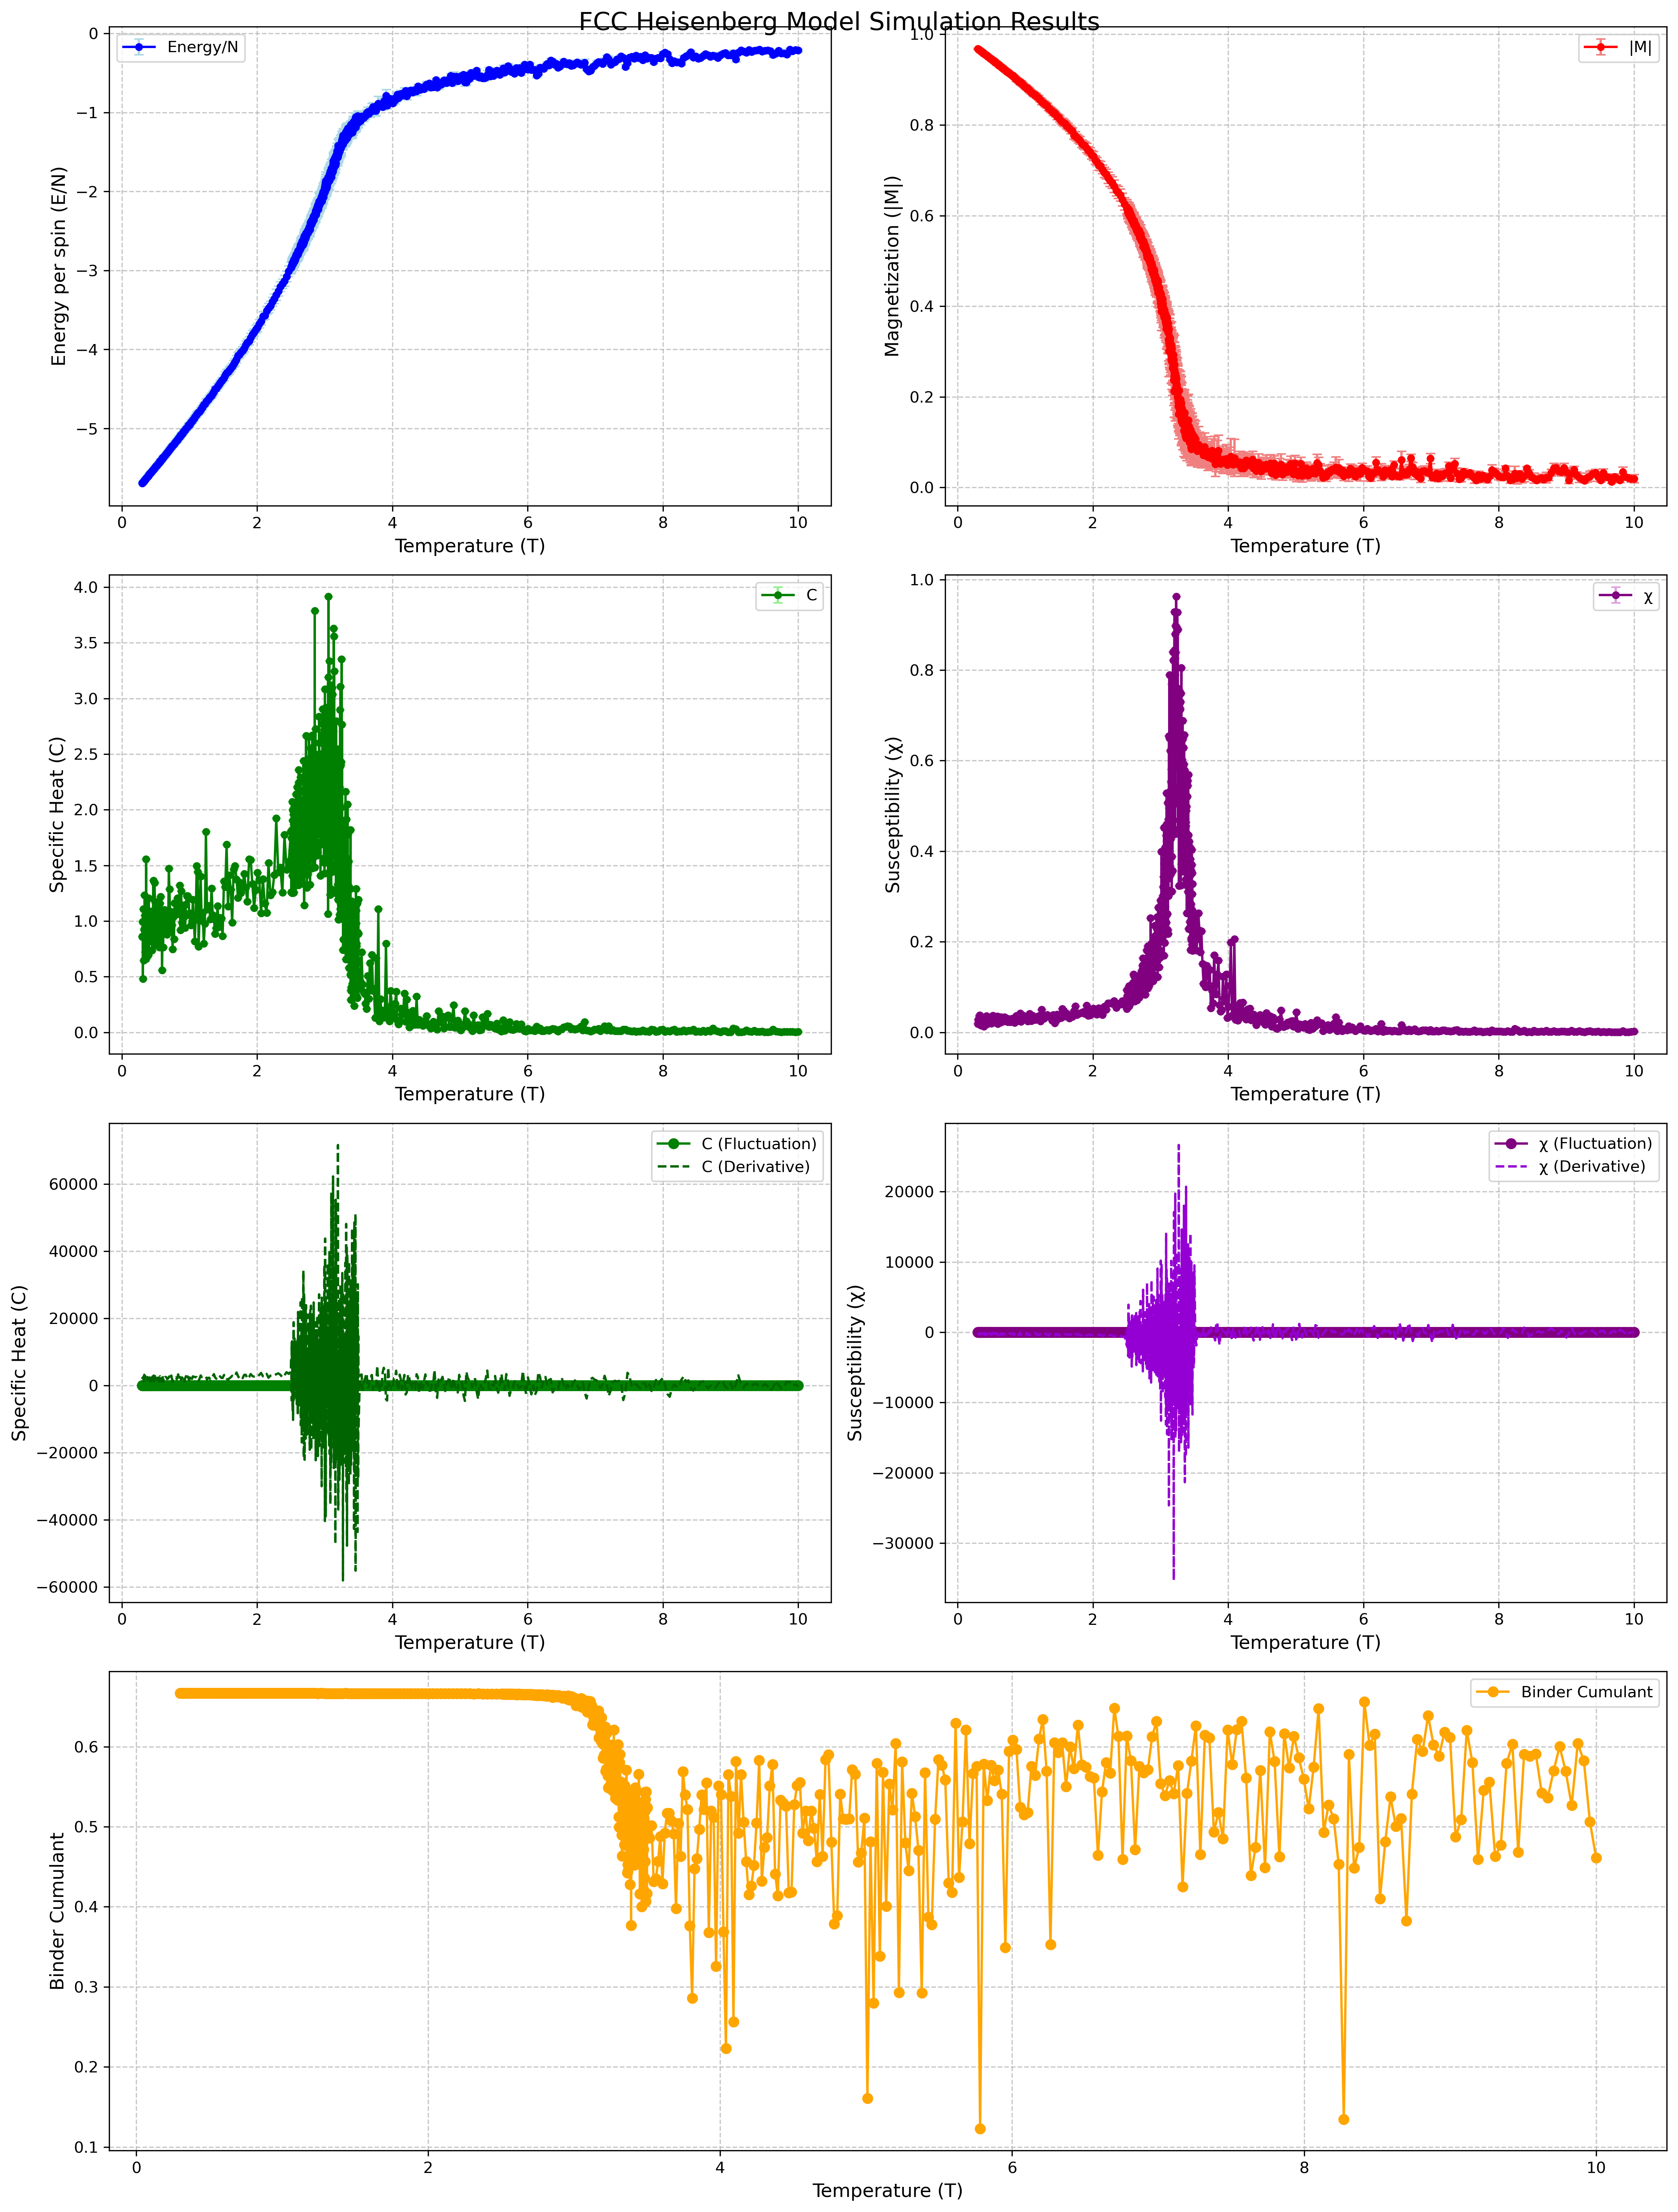
\includegraphics[width=0.85\textwidth]{Problem_2/figs/results.png}
    \caption{大规模测试结果，采用Wolff更新，$8\times8\times8$ 个 cell，每个 cell 4 个自旋，从 10 模拟退火到 0.1，1000 个温度点，每个点 200 热化（临界区翻倍）+ 1000mcs 采样}
\end{figure}
